\chapter{}
\label{Appen:A}
In that appendix we discuss a couple of things that for different reasons are only mentioned in the main document, but can still be interesting.
\section{Motor Issues: Solution Attempts}
As we discussed in \ref{subs:firstModel:issues}, we had to face many issues with the Dynamixel AX-12+ servos. Many solutions were implemented before the right one, which is explained in the thesis. Here we give an overview of all those attempts as, even if none of them completely solved our issues, developing them and understand why they were not working was a huge part of that thesis work, so they are worth to be mentioned. Here comes a brief list:
\paragraph{ROS Library:} changing the library for ROS, using both official and unofficial. It did not help because as, how it turned out later, we had a driver problem;
\paragraph{Wheel Mode vs Joint Mode:} those servos have the possibility to directly control their velocity (wheel mode) and not their position (joint mode, default behaviour). Thus, we implemented an open loop controller in wheel mode: that means that we compute for how long the motor must move at a certain speed to reach a given position. That was possible thanks to an external library, but it turned out that Dynamixels AX-12+ does not have a true speed controller, but just a PWM controller. That makes even harder to control the motors, as one would have to be able to compute how much power is needed to move the motor at a certain speed under certain conditions (e.g. load);
\paragraph{PID Controller:} again using wheel mode, we tried to build a PID controller, but since the communication with the turret was very slow, that did not improve things;
\paragraph{PID, Joint Mode:} we even tried a PID controller in joint mode, though it did not make much sense;
\paragraph{Compliance Slope and Margin:} those servos have two internal parameters. \emph{Compliance} is to set the control flexibility of the motor.
Diagram in figure \ref{fig:compliance} shows the relationship between output torque and position of the motor. \emph{Compliance Margin} exists in each direction of \acs{CW}/\acs{CCW} and means the error between goal position and present position. The greater the value, the more difference occurs. \emph{Compliance Slope} sets the level of Torque near the goal position, the higher the value, the more flexibility is obtained.
\begin{figure}
	\centering
	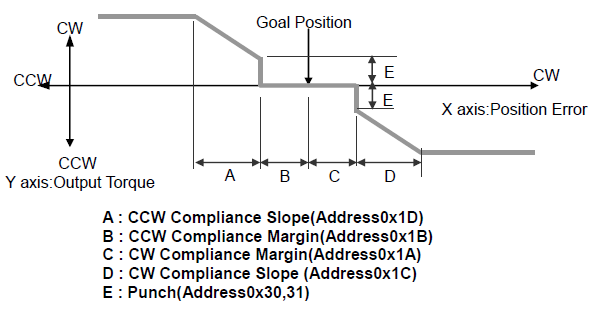
\includegraphics[width=\textwidth]{img/compliance.png}%
	\caption{Compliance Slope and Margin}
	\label{fig:compliance}
\end{figure}
Changing those values allowed us to obtain smoother trajectories, but sacrificing precision which, at the earlier stage was not important and not visible, but it could not be tolerate when implementing the relative localization system, as being imprecise with the laser pointer directly affects system performances.


\section{Motor Frames Mounting Instructions}
For sake of completeness, we include the instructions followed to mount the motors together.

Figure \ref{fig:axMounting2} shows how the \texttt{F3} is used to attach two dynamixels AX-12 together. In that way, we implement our pan component, since the bottom motor (the one on the left in the picture) can rotate the base of the upper one. Figure \ref{fig:s101Mounting} shows how the same thing can be obtained with two MX-64 servos and a \texttt{SR05-H101} frame.
\begin{figure}
	\centering
	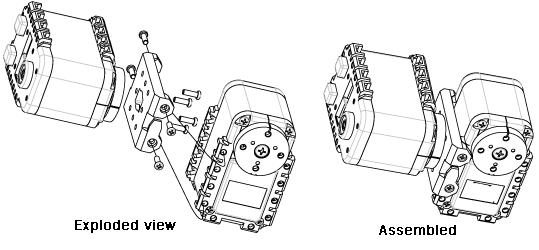
\includegraphics[width=.7\textwidth]{img/axMounting2.png}%
	\caption{Mounting F3 Frame}
	\label{fig:axMounting2}
\end{figure}
\begin{figure}
	\centering
	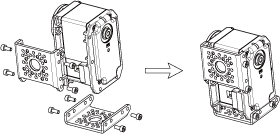
\includegraphics[width=.7\textwidth]{img/rx-64_fr05-s101.png}%
	\caption{Mounting FR05-S101 Side Frame}
	\label{fig:s101Mounting}
\end{figure}

Figure \ref{fig:axMounting1} shows how to mount the \texttt{F2} frame on top of a AX-12 servo. This is the physical representation of our tilt angle, as we mount the laser diode exactly in the middle of that frame. This is very convenient since, as already discussed, mounting the laser in that way simplifies the inverse kinematic very much. Figure \ref{fig:h101Mounting} shows the same with a \texttt{FR05-H101} hinge frame and a MX-64 motor. Note that since that frame is slightly shorter than the \texttt{F2} counterpart, we have to mount laser differently on that motor, obtaining a different and a bit more complex inverse kinematic
\begin{figure}
	\centering
	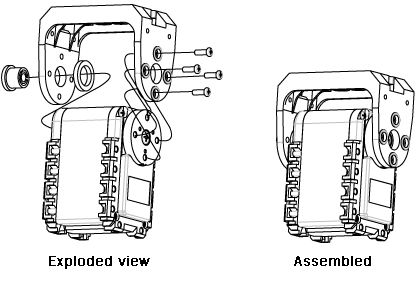
\includegraphics[width=.7\textwidth]{img/axMounting1.png}%
	\caption{Mounting F2 Frame}
	\label{fig:axMounting1}
\end{figure}


\begin{figure}
	\centering
	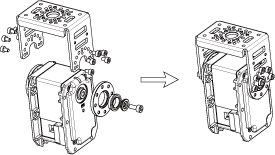
\includegraphics[width=.7\textwidth]{img/rx-64_fr05-h101.png}%
	\caption{Mounting FR05-H101 Hinge Frame}
	\label{fig:h101Mounting}
\end{figure}

\section{Data Analysis Pipeline}
In the experiment section in chapter \ref{chap:4} we analyze and report the result obtained with our experiments. Here we want to describe the pipeline built to collect those data, put them together and analyze them.

Of course, the main part regard data collection. Thank to ROS, we were able to recorder entire sessions from each user. \textit{Entire} means that we can store in bag files every single message sent through ROS and then analyze the data offline or even replay the entire experiment.

From the collected bag file, we extract all the messages relevant for the experiment and store them as \texttt{pandas} dataframes. For that, a library was provided.

Here are the main topics extracted for each experiment:

\textbf{pointing experiment}:
\begin{itemize}
    \item \texttt{arm\_pointer}, containing estimated 3D points on the ground pointed by the human (in human frame);
    \item \texttt{laser\_point}, containing 3D points of the laser dot;
    \item \texttt{target\_point}, containing 3D points of the targets on the ground (published just for convenience);
\end{itemize}
\textbf{relloc experiment}:
\begin{itemize}
    \item \texttt{relloc\_human\_pose}, containing estimated 3D points of the human in the turret frame, computed and published for application purposes;
    \item \texttt{gt\_point}, containing 3D ground truth points, i.e. the points where the user should stand when doing the relloc. We need to publish since they are randomly shuffled for each user, thus we cannot assume that we already know them.
\end{itemize}
Given that, is easy to understand how we obtain the results discussed in chapter \ref{chap:4}. For the pointing experiment, we confront \texttt{arm\_pointer} points with \texttt{laser\_point} ones, considering also their distances from the targets for each session. For the relloc one, for each session we compute the distance between the ground truth point and the estimated one.

It is also worth to say that the aforementioned concept of \textit{session} needed a bit of work to be implemented, as each dataframe needed to be parsed and each session distinguished from the others. To do that easily, we implemented a machine state mechanism which publishes a string message over a ROS topic containing the current state of the system. With a clever use of that concept, we are able to mark the begin and the end of each session and then recover it when parsing the data.

To conclude, we can add that the code to parse the data, analyze and print/plot results is available as convenient \texttt{ipython} notebooks. In that way, we can easily run and analyze new data eventually collected.